\section{High Level Considerations}

Before diving into the details of consensus mechanisms, let's take a look at the advantages and limitations of using blockchain:

% \begin{table}[h!]
% \centering
% \begin{tabular}{|p{0.45\textwidth}|p{0.45\textwidth}|}
% \hline
% \rowcolor{Blue}
% \textbf{\color{white}Benefits} & \textbf{\color{white}Limitations} \\
% \hline
% Decentralization & New Technology \\
% Transparency and Trust & Scalability \\
% Immutability and Privacy & Confidentiality \\
% High Availability & Limited Adoption \\
% High Security & Interoperability \\
% Process Optimization and Simplification & Regulation \\
% Quick settlement & \\
% Cost savings & \\
% Reliable application platform & \\
% Programmable properties & \\
% \hline
% \end{tabular}
% \caption{Benefits and Limitations of Blockchain Technology.}
% \end{table}

\begin{table}[ht]
\noindent\begin{minipage}[t]{0.45\textwidth}
\centering
\begin{tabular}{|p{\textwidth}|}
\hline
\rowcolor{Blue!90}
{\textbf{\color{white}Benefits}} \\
\hline
Decentralization \\
Transparency and Trust \\
Immutability \\
High availability \\
Highly secure \\
Simplification of processes \\
Quick settlement  \\
Cost-saving \\
Trusted application platform \\
Programmable property \\
\hline
\end{tabular}
\end{minipage}\hfill
\begin{minipage}[t]{0.45\textwidth}
\centering
\begin{tabular}{|p{\textwidth}|}
\hline
\rowcolor{Blue!90}
{\textbf{\color{white}Limitations}}\\
\hline
New technology \\
Scalability \\
Privacy and confidentiality \\
Limited Adoption \\
Interoperability \\
Regulation \\
\\
\\
\\
\\
\hline
\end{tabular}
\end{minipage}
\caption{Benefits and Limitations of Blockchain Technology.}
\end{table}

\section{DLT Categories}
\textbf{Distributed Ledger Technologies} (DLTs) can be categorized in different ways based on their use and structure. One of the main categories is Blockchain, which is a specific type of DLT used for shared and immutable ledgers.

\begin{figure}[h]
\centering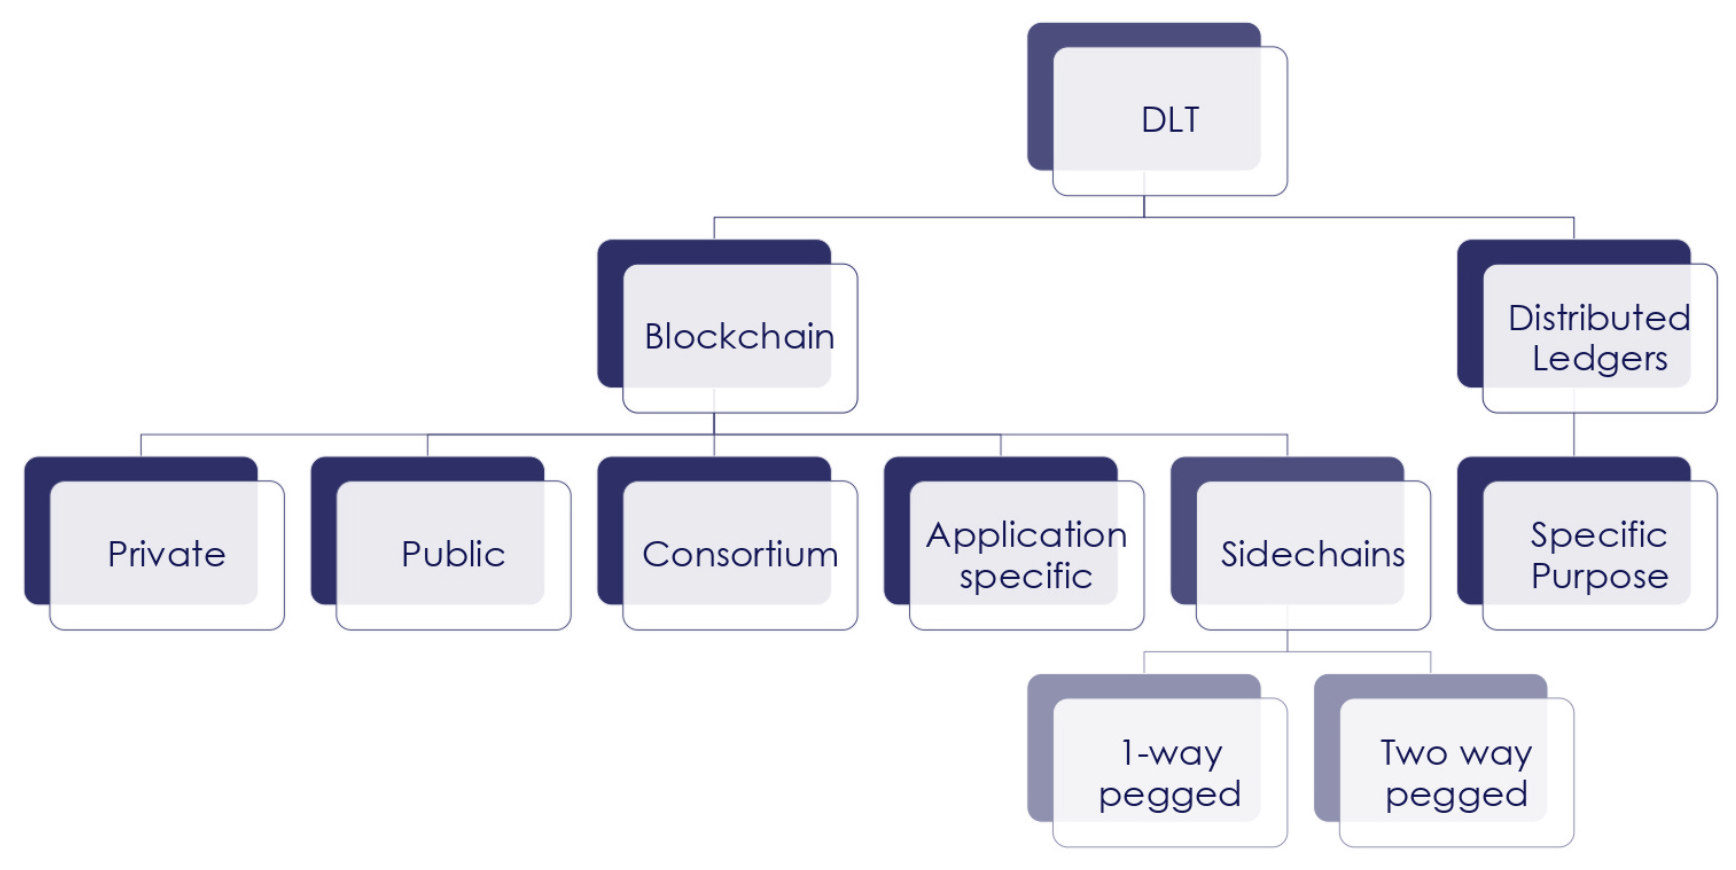
\includegraphics[scale=0.3]{images/chapter3 - DLT.png}
\caption{Distributed Ledger Technologies Categories.}
\end{figure}

Blockchain can be further divided into three main types: public, private and consortium. \textbf{\textcolor{Orange}{Public blockchains}} are open to anyone who wants to participate and are decentralized. \textbf{\textcolor{Orange}{Private blockchains}} are controlled by a centralized organization or entity and are accessible only to authorized users. \textbf{\textcolor{Orange}{Consortial blockchains}} are managed by a group of organizations working together to manage the network.

In addition to blockchains, there are other types of DLTs such as Sidechains and Distributed Ledgers. \textbf{\textcolor{Orange}{Sidechains}} are blockchains linked to a main blockchain and can be used for specific purposes or to enhance the functionality of the main blockchain. \textbf{\textcolor{Orange}{Distributed Ledgers}}, on the other hand, are shared ledgers that can be customized for specific purposes and are not necessarily blockchain-based.
